\subsection{Single Star Evolution}\label{sec:SingleStarEvolution}

\subsubsection{Class Hierarchy}\label{sec:SSEClassHierarchy}

The SSE architecture is based on the classification of individual stars, with each stellar classification being described by a separate C++ class. Figure~\ref{fig:SSE_ClassDiagram} shows the SSE class diagram, where the arrows indicate inheritance.  The COMPAS C++ code is implemented using multiple inheritance, and all stellar classes also inherit directly from the Base Star class (arrows not shown in Figure~\ref{fig:SSE_ClassDiagram} for clarity). Each of the stellar classes encapsulates data structures and algorithms specific to the evolutionary phase corresponding to the class.

The main class for single star evolution is the \textbf{Star} class. The Star class is a wrapper that abstracts away the details of the star and the evolution.  Internally the Star class maintains a pointer to an object representing the star being evolved, with that object being an instance of one of the following classes:

\bigskip
\hfill
\begin{minipage}{\dimexpr\textwidth-2em}
    \textbf{MS\_lte\_07} \\
    \textbf{MS\_gt\_07} \\
    \textbf{CH} \\
    \textbf{HG} \\
    \textbf{FGB} \\
    \textbf{CHeB} \\
    \textbf{EAGB} \\
    \textbf{TPAGB} \\
    \textbf{HeMS} \\
    \textbf{HeHG} \\
    \textbf{HeGB \\}
    \textbf{HeWD} \\
    \textbf{COWD} \\
    \textbf{ONeWD} \\
    \textbf{NS} \\
    \textbf{BH} \\
    \textbf{MR} \\
\end{minipage}

which track the phases from \citet{Hurley_2000}, with the exception of the \textbf{CH} class for Chemically Homogeneous stars, which is not described in \citet{Hurley_2000}.

Several other SSE classes are defined:

\bigskip
\hfill
\begin{minipage}{\dimexpr\textwidth-2em}
    \textbf{BaseStar} \\
    \textbf{MainSequence} \\
    \textbf{GiantBranch} \\
    \textbf{Remnants} \\
    \textbf{WhiteDwarfs}
\end{minipage}
 
\bigskip
These extra classes are included to allow inheritance of common functionality.

The \textbf{BaseStar} class is the main class for the underlying star object held by the Star class.  The BaseStar class defines all member variables, and many member functions that provide common functionality.  Similarly, the \textbf{MainSequence} and \textbf{GiantBranch} classes provide repositories for common functionality for main sequence and giant branch stars respectively, and the the \textbf{Remnants} and \textbf{WhiteDwarfs} classes provide repositories for common functionality for remnant and white dwarf stars respectively.

\begin{figure}
    \begin{center}
	    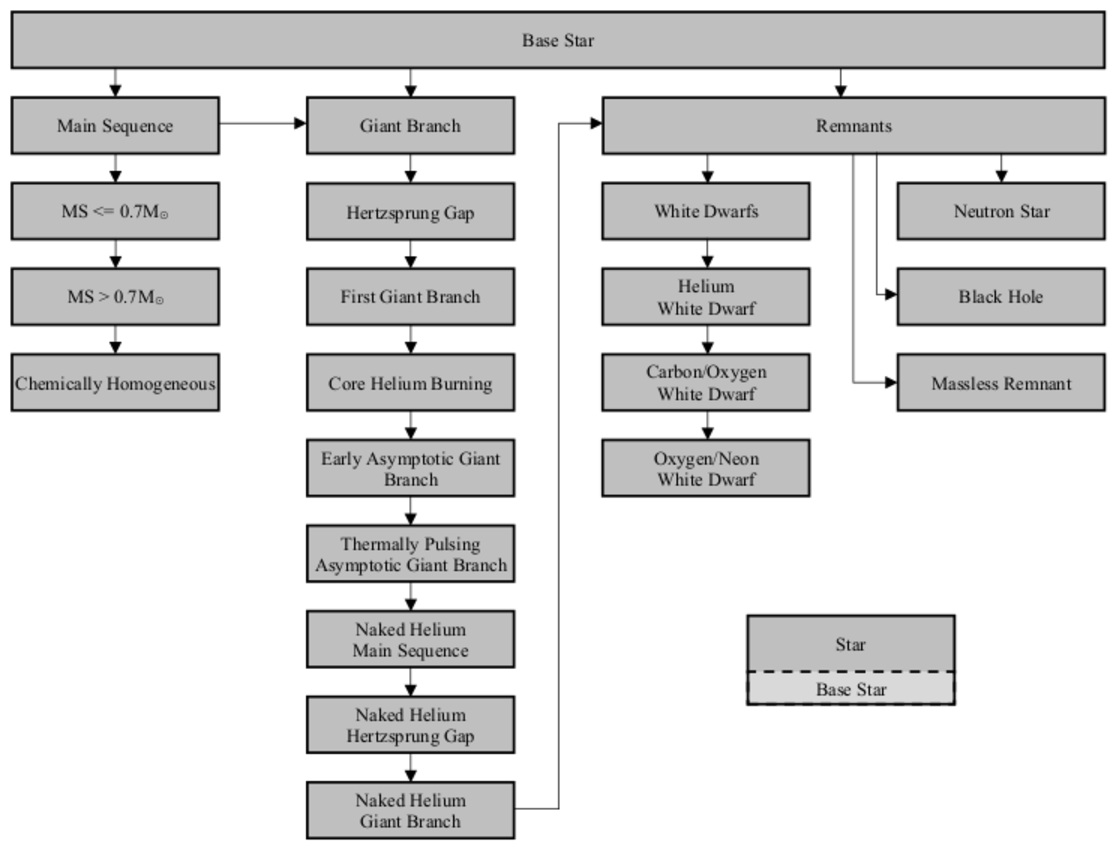
\includegraphics[viewport = 0 0 535 405, width = 13.65cm, clip]{sections/images/SSE_ClassDiagram.pdf}
    \end{center}
    \vspace{-2.00mm}
    \caption{SSE class diagram.}
    \label{fig:SSE_ClassDiagram}
\end{figure}

\medskip
\textbf{CH} (Chemically Homogeneous) class stars inherit from the \textbf{MS\_gt\_07} class because (in this implementation) they are just (large) main sequence stars that have a static radius.

\textbf{HG} (Hertzsprung Gap) class stars inherit from the GiantBranch class because they share the giant branch parameters described in \citet{Hurley_2000}, section 5.2.

Each class has its own set of member functions that calculate various attributes of the star according to the phase the class represents (using the equations and parameters from \citet{Hurley_2000} where applicable).

\newpage
\subsubsection{Evolution Model}\label{sec:SSE_EvolutionModel}

The high-level stellar evolution model is shown in Figure~\ref{fig:SSE_FlowChart}.

\begin{figure}
    \begin{center}
	    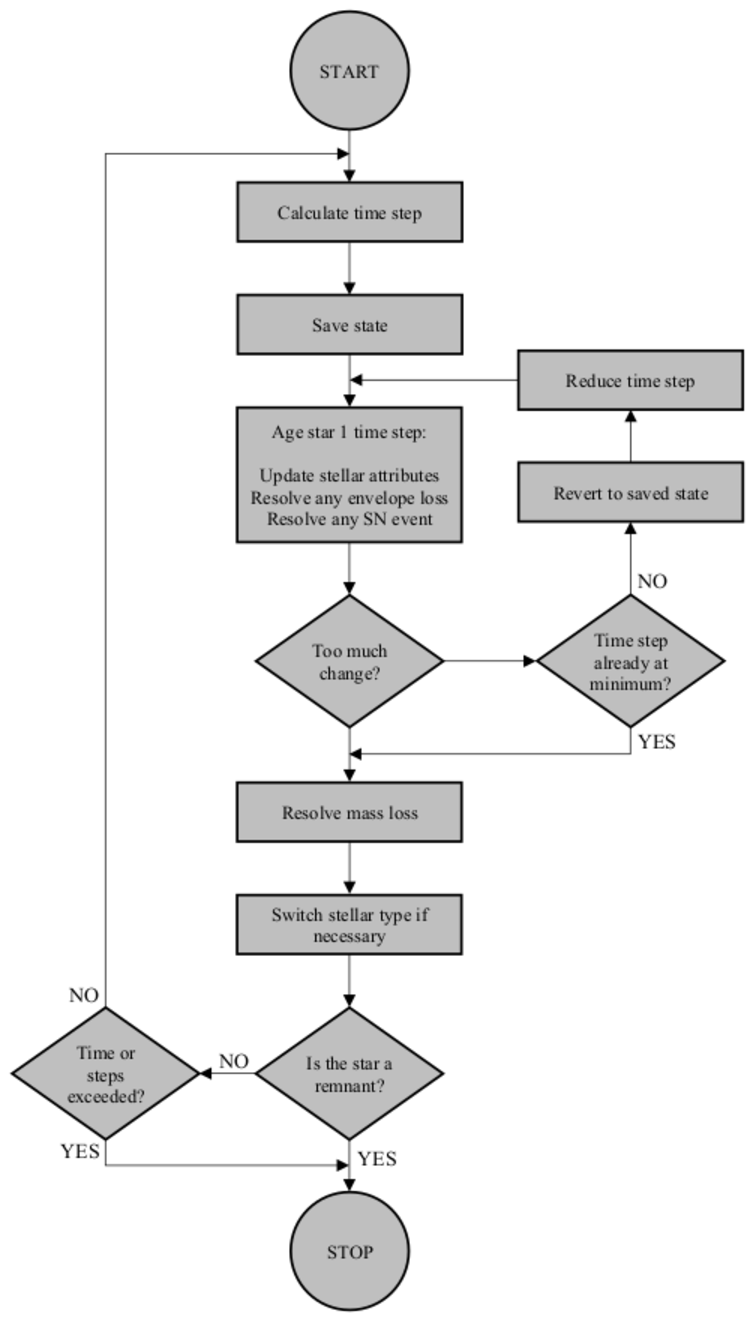
\includegraphics[viewport = 0 0 360 632, width = 8.5cm, clip]{sections/images/SSE_FlowChart.pdf}
    \end{center}
    \vspace{-2.00mm}
    \caption{High-level SSE evolution.}
    \label{fig:SSE_FlowChart}
\end{figure}

\newpage
The stellar evolution model is driven by the \textbf{Evolve()} function in the Star class, which evolves the star through its entire lifetime by doing the following:

\tabto{2em}DO:

\hfill
\begin{minipage}{\dimexpr\textwidth-4em}
    \begin{enumerate}
        \item {
            calculate time step
            \begin{enumerate}
                \item {calculate the giant branch parameters (as necessary)}
                \item {calculate the timescales}
                \item {choose time step}
            \end{enumerate}
        }
 
        \item {save the state of the underlying star object}

        \item {
            DO:

            \hfill
            \begin{minipage}{\dimexpr\textwidth-4em}
                \begin{enumerate}
                    \item {evolve a single time step}
                
                    \item {
                        if too much change
                        \begin{enumerate}
                        \item{revert to the saved state}
                        \item{reduce the size of the time step}
                        \end{enumerate}
                    }
                \end{enumerate}
            \end{minipage}

            UNTIL timestep not reduced
        }
  
        \item {
            resolve any mass loss
            \begin{enumerate}
                \item {update initial mass (mass0)}
                \item {update age after mass loss}
                \item {apply mass transfer rejuvenation factor}
            \end{enumerate}
        }
 
        \item { evolve to the next stellar type if necessary }

    \end{enumerate}
\end{minipage}

\bigskip
\tabto{2em}WHILE the underlying star object is not one of: \lcb\ HeWD, COWD, ONeWD, NS, BH, MR\ \rcb

\bigskip
\bigskip
Evolving the star through a single time step (step 3a above) is driven by the \nobreak\textbf{UpdateAttributesAndAgeOneTimestep()} function in the BaseStar class which does the following:

\begin{enumerate}
    \item {check if the star should be a massless remnant}
    \item {check if the star is a supernova}
\end{enumerate}

\tabto{1.2em}if evolution on the phase should be performed

\hfill
\begin{minipage}{\dimexpr\textwidth-2em}
    \begin{enumerate}
        \setcounter{enumi}{2}
        \item  evolve the star on the phase -- update stellar attributes
        \item  check if the star should evolve off the current phase to a different stellar type
    \end{enumerate}
\end{minipage}

\medskip\tabto{1.2em}else

\hfill
\begin{minipage}{\dimexpr\textwidth-2em}
    \begin{enumerate}
        \setcounter{enumi}{4}
        \item  ready the star for the next time step
    \end{enumerate}
\end{minipage}

\newpage
Evolving the star on its current phase, and off the current phase and preparing to evolve to a different stellar type, is handled by two functions in the BaseStar class: \textbf{EvolveOnPhase()} and \textbf{ResolveEndOfPhase()}.

The EvolveOnPhase() function does the following:

\medskip
\hfill
\begin{minipage}{\dimexpr\textwidth-2em}
\begin{enumerate}
    \item  Calculate Tau
    
    \item  Calculate CO Core Mass \\
    \item  Calculate Core Mass \\
    \item  Calculate He Core Mass \\

    \item  Calculate Luminosity \\
    \item  Calculate Radius

    \item  Calculate Perturbation Mu \\
    \item  Perturb Luminosity and Radius

    \item  Calculate Temperature

    \item  Resolve possible envelope loss
\end{enumerate}
\end{minipage}

\bigskip
Each of the calculations in the EvolveOnPhase() function is performed in the context of the star evolving on its current phase.  Each of the classes implements their own version of the calculations (via member functions) -- some may inherit functions from the inheritance chain, while others might just return the value unchanged if the calculation is not relevant to their stellar type.

\newpage
The ResolveEndOfPhase() function does the following:

\medskip
\hfill
\begin{minipage}{\dimexpr\textwidth-2em}
    \begin{enumerate}
        \item  Resolve possible envelope loss

        \item  Calculate Tau

        \item  Calculate CO Core Mass \\
        \item  Calculate Core Mass \\
        \item  Calculate He Core Mass

        \item  Calculate Luminosity \\
        \item  Calculate Radius

        \item  Calculate Perturbation Mu \\
        \item  Perturb Luminosity and Radius

        \item  Calculate Temperature

        \item  Evolve star to next phase
    \end{enumerate}
\end{minipage}

\bigskip
Each of the calculations in the ResolveEndOfPhase() function is performed in the context of the star evolving off its current phase to the next phase.

The remainder of the code (in general terms) supports these main driver functions.
